\documentclass[12pt]{article}
\title{Discouragement Attacks}
\author{
        Vitalik Buterin \\
        Ethereum Foundation
}
\date{\today}
\usepackage{graphicx}


\begin{document}
\maketitle
\begin{abstract}
We explore ``discouragement attacks" on economic consensus mechanisms. A discouragement attack consists of an attacker acting maliciously inside a consensus mechanism in order to reduce other validators' revenue, even at some cost to themselves, in order to encourage the victims to drop out of the mechanism. The motivations to conduct discouragement attacks are twofold. First, the attacks can increase the attacker's profit, as the mechanism may contain ``competitive" dynamics where some validators dropping out increases revenue to the remaining ones. Second, the attacks can be part of a two-step strategy where the second step is to carry out a traditional $51\%$ attack on the consensus algorithm against a now much smaller set of ``honest" validators warding off the attacker, and hence pay a much lower cost for the attack.
\end{abstract}

\section{Introduction}
Consider the following type of attack on a proof of stake blockchain. The rules of the chain are as follows: there is a maximum total reward $R$, and if there are $N$ validators (consider each validator as having deposited one coin) then each validator, during every 10-second slot, has a chance to earn a reward of $\frac{R}{N}$ if they actually sign a message that contributes to the chain's consensus during that round. An attacker that controls $\frac{N}{2} + 1$ validators starts refusing to include messages from all remaining validators. Initially, the attack reduces the victims' revenue to zero and leaves the attacker's revenue unchanged. However, the victims then see no incentive to continue to be validators and exit the proof of stake mechanism. The validator count reduces to $\frac{N}{2} + 1$, and the attacker's revenue increases from $R * \frac{\frac{N}{2} + 1}{N}$ to $R$.

Here is a possible alternative ending: once everyone but the attacker leaves, the attacker slowly exits their validators until only one validator remains. They then perform a double-spending attack, censorship attack or any other kind of attack on the chain. In either case, it's clear that this kind of two-step strategy is potentially a much cheaper way of bringing down blockchains than a direct frontal attack.

\section{Griefing factors}

To analyze attacks like these, a common tool that we use is the \emph{griefing factor}. A mechanism in some equilibrium has a griefing factor of $N$ if the attacker has a mechanism by which they can sacrifice \$1 of their own funds to cause \$N of losses to the other participants. If attackers can harm others costlessly or profitably, the griefing factor is $\infty$. With respect to attackers with $\ge \frac{1}{2}$ of all validators, the toy proof of stake mechanism we described above has griefing factor $\infty$.

However, it is possible to modify the mechanism to bound the griefing factor: if $M$ out of $N$ validators are seen signing a message, then each validator that signs only earns $\frac{R}{N} * \frac{M}{N}$. Then, if the possibility of victims withdrawing or depositing is not taken into account, an attacker with $\frac{N}{2}$ validators censoring $k$ validators (for simplicity of analysis we'll assume that 51\% attacks are possible with exactly 50\%) cuts the reward of all online validators from $\frac{R}{N}$ to $\frac{R}{N} * \frac{N-k}{N}$, and so causes:

\begin{itemize}
\item $\frac{N}{2} * \frac{R}{N} * \frac{k}{N} = R * \frac{k}{2N}$ losses to themselves due to reward reduction
\item $\frac{R}{N} * k = R * \frac{k}{N}$ losses to victims of censorship
\item $(\frac{N}{2} - k) * \frac{R}{N} * \frac{k}{N} = R * (\frac{k}{2N} - \frac{k^2}{N^2})$ losses to others due to reward reduction 
\end{itemize}

As $k$ approaches zero, the griefing factor approaches $\frac{R * \frac{k}{N} + R * \frac{k}{2N}}{R * \frac{k}{2N}} = 3$. As $k$ approaches $\frac{N}{2}$, the griefing factor approaches $\frac{\frac{k}{N}}{\frac{k}{2N}} = 2$. Minorities can also grief majorities by going offline, and for a minority attacker the griefing factor is limited to $1$ for small attacks and $\frac{1}{2}$ for attacks with size approaching half the entire validator set. In the rest of our analysis, we will speak abstractly about proof of stake mechanisms with particular griefing factors; this will allow us to compartmentalize our analysis.

\section{Epsilon attacks}

We will start off examining a particular subclass of attack, where the extent of the attack is small. That is, the attacker selectively censors or otherwise interferes with a small portion of the messages of the victims, reducing their rewards but not enough to make them all leave.

In our naive examples above, the reward given to each validator was a $\frac{1}{N}$ share of some fixed total pot, $R$, where $N$ is the total number of validators (or total deposit size). But this is really only one policy among many possible policies. We can categorize many of them with the equation $r = N^{-p}$, where:

\begin{itemize}
\item $p=0$: constant ``interest rate", eg. under optimal conditions each validator earns a return of $8\%$ per year.
\item $p=\frac{1}{2}$: the rewards (and penalties) to validators scale with $\frac{1}{\sqrt{N}}$, so \textit{total} rewards scale with $\sqrt{N}$. This is a compromise between $p=0$ and $p=1$. 
\item $p=1$: constant total reward, ie. the total payout of the protocol is dependent only on what percentage of validators take what actions, not on the total deposit size.
\item $p=\infty$: the protocol is dead-set on ensuring that the total deposit size is some specific constant $N_k$ no matter what. If the total deposit size exceeds $N_k$, the protocol keeps decreasing rewards until it drops to $N_k$, and if the total deposit size is below $N_k$, the protocol keeps increasing rewards until it rises to $N_k$. Mathematically, we represent this as the reward curve being a vertical line at $x = N_k$, being equal $\infty$ below $N_k$ and $0$ above $N_k$.
\end{itemize}

Note that if revenues to validators are dominated by transaction fees, then $p=1$ will hold.

We now rephrase the problem into the language of supply and demand: there exist a set of players, each of which has some \textit{reserve reward level} at which they are willing to become validators in the consensus mechanism. This is the supply curve, where the reward level is the price. The protocol, which offers rewards for participation in the consensus mechanism, sets the demand curve. If $p=0$, the demand curve is horizontal - the protocol offers that interest rate to an unlimited number of validators. If $p=\infty$, the demand curve is vertical. For any other $p$, the demand curve is declining diagonally. For simplicity, we will suppose that the supply curve is $N = r^k$ for some $k$ (eg. $k = 1$) where $r$ is the per-validator reward offered. Absent any attacks, the status-quo values of $N$ and $r$ are the intersection of the supply curve offered by potential validators and the demand curve offered by the protocol.

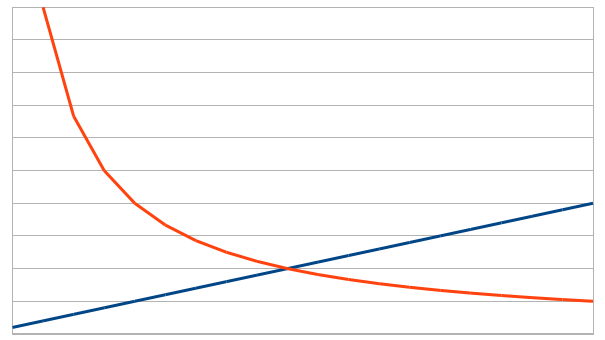
\includegraphics[width=300px]{disc_chart1.png}

We model an attack as \emph{pushing the entire demand curve down}, and in addition costing or benefiting the attacker. We can determine everyone's equilibrium profit by calculating the intersection of the (unchanged) supply curve and the new (depressed) demand curve, and then adding a term to take into account the fact that the attacker's profits as a percentage of their deposits may be less or more than everyone else's.

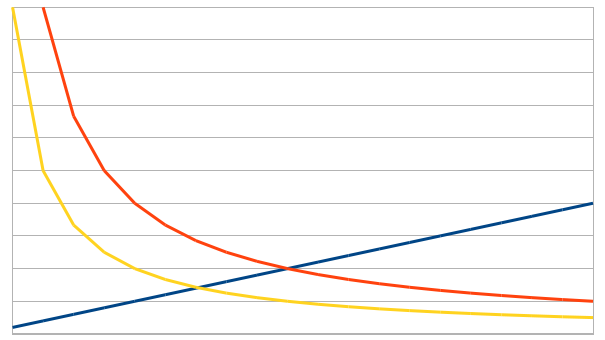
\includegraphics[width=300px]{disc_chart2.png}

Locally, we can see the protocol reward curve as a straight line with slope $-p$, and the supply curve of users' willingness to participate as a straight line with slope $k$. If the reward curve is pushed down by $\epsilon$, then the validator count is pushed left by $\frac{\epsilon}{k+p}$ and the reward is reduced by $\epsilon * \frac{k}{k + p}$ (another way to think about it is that everyone loses $\epsilon$ from the attack and then \emph{recovers} $\frac{p}{k+p}$ from the equilibrium shifting left). Hence, for example, if $k = p = 1$, then because of the marginal validators the attack drives away, everyone (including victims and attacker) earns back an amount equal to half the original per-validator loss of each victim. If $k = 1$ and $p = \frac{1}{2}$, then everyone only earns back a third.

Note that the analysis does not change if the attacker makes a targeted attack, provided the attacker does not have special knowledge about the victim's willingness to be a validator (to preserve this assumption, we generally recommend proof of stake validators try to remain anonymous). The reason is that an attack on $\frac{1}{M}$ of the validator set with the same griefing factor harms them $M$ times as much, driving $M$ times as many to leave, but the set affected is only $\frac{1}{M}$ in size, so on net the same number of victims leave as a result of the attack.

Griefing factors are highest when the attacker has exactly half of the validators. This is convenient, because it means that the size of the attacker and victim sets are the same, so the griefing factor is also the ratio of the losses of average rewards \emph{of each validator}. Let us suppose the victims lose $\epsilon$. If the mechanism has a griefing factor of $N$, then the attacker loses $\epsilon * \frac{1}{N}$. If everyone recovers $\epsilon * r$ where $r = \frac{p}{k+p}$, then the victims' losses become $\epsilon * (1-r)$ and the attacker's losses $\epsilon * (\frac{1}{N} - r)$. Hence, an attack can be profitable if $\frac{p}{k+p} > \frac{1}{N}$.

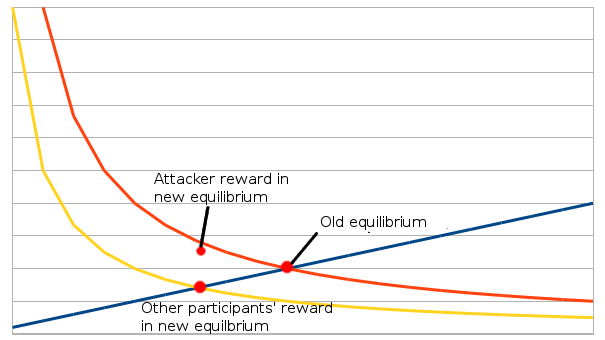
\includegraphics[width=300px]{disc_chart3.png}

If $N = 3$, as is the case in the simplest collective-penalty scheme described above, and we assume $k=1$, then this implies we need $p \le \frac{1}{2}$ for epsilon attacks to be unprofitable.

\section{Total attacks}

Attackers with less than 50\% of the validator set, or attackers trying to make the attack \emph{look} innocuous (eg. passing it off as abnormally high network latency) only have epsilon attacks at their disposal. An epsilon attack has the disadvantage that the attack must keep running, continuing to cost the attacker. But what if the attacker can drive \emph{everyone} out (eg. attack enough to push victims' revenues to below zero)? Then, from inside the mechanism, it looks as though no one is attacking (as all victims are no longer participating), and so the attacker is claiming their full maximum rewards. In fact, if $p > 0$, the attacker is claiming \emph{more} rewards than before.

Additionally, unlike epsilon attacks, total attacks can be used to drive the cost of doing an outright attack on the chain (eg. reverting finality) down to zero, although only blocks finalized after the non-attacking validators all leave can be reverted cheaply, so it may be philosophically more correct to consider such an attack an attack on \emph{liveness} rather than \emph{safety}.

One answer may be: if a total attack, driving the revenues of innocent validators to below zero, is taking place, clients can detect this, and coordinate a minority soft fork extra-protocol to remove the attacker. But can we do better?

We could choose $p < 0$ to make such attacks greatly unprofitable; however, this imposes great instability on the protocol because small shifts in demand for validating could lead to very large shifts in both the size of the validator set and the total issuance; indeed, as $p$ approaches $-k$ arbitrarily small shifts in demand can cause arbitrarily large shifts in validator set size. Hence, such an approach is likely nonviable.

Another approach is to limit the rate at which validators exit, making it difficult for many validators to leave at the same time. This would require an attacker to sustain an attack for a longer period of time, during which the community could mount a response, and costing the attacker more in the meantime. Particularly, one could freeze all validator withdrawals for the entire period during which the protocol detects that there is an attack and validators are not earning money. An attacker could still attack at zero cost in a richer economic model by \emph{precommitting} to attack and letting other validators leave first, but this would be more complicated to implement.

Finally, one can add an ``assurance contract'' mechanic into the deposit mechanism: a validator wishing to enter can specify the minimum validator set size at which they are willing to enter (eg. if there are 1000 validators currently in the validator set one could specify $\le 1000$ to enter immediately or one could specify 1500). The deposit mechanism would try to induct as many validators as possible such that every validator would satisfy its constraint (eg. if there are currently 1000 validators waiting, and new validators want to join with specified minimums 1001 1003 1004 1004 1006, then the first four could be inducted, as that would increase the count to 1004 which would satisfy all four of them, but the remaining one would not be inducted as if all five joined the total validator count would become 1005, and $1005 < 1006$. This would allow validators to more easily coordinate to fight back against attacks, effectively by saying ``I'm willing to join only if enough others join at the same time to defeat this attacker with me".

\section{Conclusion}

Discouragement attacks as a cheaper way of attacking a consensus algorithm are one of the hardest classes of attacks to come up with defenses against. This is even more true in proof of work: if a 51\% attack succeeds, then there is a coordination problem opposing ``honest" miners trying to recover the original fork, as none have the private incentive to participate in a fork unless everyone else does. There are some possible strategies for mitigating these attacks especially in a proof of stake system, including making them take longer to execute, easier to coordinate to defeat, and less profitable, but none are perfect. In general, this is still an active area of research, and more research on counter-strategies is desired.

\bibliographystyle{abbrv}
\bibliography{main}

\end{document}
